\documentclass[11pt,a4paper]{article}

%
% $Id: howtobuild.tex,v 1.14 2006/04/25 14:20:24 schnelle Exp $
%

\usepackage[latin1]{inputenc}
\usepackage{graphics}
\usepackage{graphicx}
\usepackage{url}
\usepackage{listings}
\usepackage{xcolor}

\title{How to build JVoiceXML \\
Version 1.6}

\author{Dirk Schnelle,  \\
  \texttt{dirk.schnelle@jvoicexml.org} } 

\date{}

\begin{document}
\pagestyle{headings}
\lstset{language=Java,language=XML,
        backgroundcolor=\color{lightgray},
        basicstyle=\small,
        numbers=left,
        numberstyle=\tiny,
        stepnumber=5}

\maketitle

\begin{abstract}
This documents describes the steps you have to perform, when you want
to build JVoiceXML or develop code for the JVoiceXML project. It gives
information about the requirements of your development environment 
and our coding conventions.
\end{abstract}

\section*{Acknowledgment}

Thanks to Adrindam Das for writing the TortoiseCVS~\cite{tortoisecvs} 
part and some screen shots.

\section{Introduction}
\label{sec:introduction}

JVoiceXML is a free VoiceXML~\cite{w3.org:voicexml} implementation written in 
the JAVA programming language. It offers a library for easy VoiceXML
document creation and a VoiceXML interpreter to process 
VoiceXML documents using JAVA standard APIs such as JSAPI~\cite{sun:jsapi} and
JTAPI~\cite{sun:jsapi}.

VoiceXML is hosted at SourceForge~\cite{sourceforge} as an open source project.
You find everything that is related to this project under
\url{http://sourceforge.net/projects/jvoicexml/}.

This document refers to UNIX and Windows systems. JVoiceXML will work 
any other operating systems that support Java 5, too.

Nobody is perfect, so you may find some errors or small things to correct.
Please let me know if you think you found something that should be written
differently.

\section{Copyright}
\label{sec:copyright}

JVoiceXML uses the GNU library general public license~\cite{gnu:lgpg}. 
This is mentioned in all our source files as a unique header, see
section~\ref{sec:code-conventions}.
You can find a copy in the file COPYING in the \$\{JVOICEXML\_HOME\}
directory. This means that you are allowed to use JVoiceXML
library in your commercial programs. If you make some nice
enhancements it would be great, if you could send us your
modifications so that we can make it available to the public.

JVoiceXML is free software; you can redistribute it and/or
modify it under the terms of the GNU Library General Public
License as published by the Free Software Foundation; either
version 2 of the License, or (at your option) any later version.

JVoiceXML is distributed in the hope that it will be useful,
but WITHOUT ANY WARRANTY; without even the implied warranty of
MERCHANTABILITY or FITNESS FOR A PARTICULAR PURPOSE. See the GNU
Library General Public License for more details.

You should have received a copy of the GNU Library General Public
License along with this library; if not, write to the Free
Foundation, Inc., 59 Temple Place, Suite 330, Boston, MA  02111-1307  USA

\section{Download the source code}

\subsection{Download the source archive}

You can download a the source code for the available releases from 
\url{http://jvoicexml.sourceforge.net/downloads.htm}.
Create a directory JVoice\-XML and unpack the zipped source file into it.
In the rest of this document this directory will be referred as
\$\{JVOICE\-XML\_HOME\}.

\begin{lstlisting}
mkdir JVoiceXML
cd JVoiceXML
unzip jvxml-src-VERSION.zip
\end{lstlisting}

\texttt{VERSION} has to be replace by the used version number, i.e. 0.5.

Note that the third party libraries are not part of this zip archive.
You should download the libraries from their original location,
download them from our cvs repository, see 
section~\ref{sec:cvs-repository}, or download the binary distribution.
All used libraries are located in the \texttt{lib} folder of
your JVoiceXML installation. Just create a directory 
\texttt{3rdparty} and copy all jars to this folder.

\begin{lstlisting}
mkdir 3rdparty
cp JVOICEXML_HOME/lib/*.jar 3rdparty
\end{lstlisting}

Note that you will have to adapt the lib properties of the build file
if you just copy the jars.

\subsection{SVN repository}
\label{sec:cvs-repository}

If you want to stay at the current state of development you have to use
the SVN repository from Source Forge~\cite{sourceforge}.
This is also the preferred way.
This section describe the parameters to access the SVN repository 
using the command line. Feel free to grab the required parameters from
this description and feed your third party tool with them.

\begin{lstlisting}
svn co https://svn.sourceforge.net/svnroot/jvoicexml jvoicexml
\end{lstlisting}

This will check out the whole repository, including the main module,
tags and branches of JVoiceXML. If you are just interested in the
main development \emph{trunc} you will have to append \texttt{/trunc} to
the HTTPS URL:

\begin{lstlisting}
svn co https://svn.sourceforge.net/svnroot/jvoicexml/trunc jvoicexml
\end{lstlisting}

\textbf{Note:} UNIX file and directory names are case sensitive.

\section{Directory structure}
\label{sec:directory-structure}

Having the source code in your \$\{JVOICEXML\_HOME\} directory you
find the following directory structure:

\begin{center}
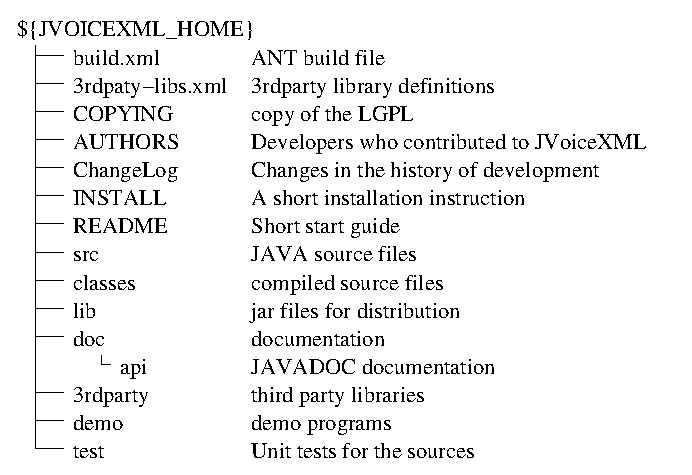
\includegraphics{structure.eps}
\end{center}

Not all of the files are present at start but are created by the
ANT build file or through procedures described in this 
document, see section~\ref{sec:ant-build-file}.

\section{Required Software}
\label{sec:required-software}

Since JVoiceXML is written in JAVA you will at least need a
JAVA compiler~\ref{sec:ide}, an editor or preferably a JAVA
IDE~\ref{sec:ide} and ANT~\ref{sec:ant} to build the binaries.
All used third party libraries can be downloaded from the CVS 
repository or from their home pages.

\subsection{IDE}
\label{sec:ide}

You can use the IDE of your choice to edit the sources and compile the 
binaries. You can even use a simple text editor to perform this job.
Nevertheless there are some restriction that you cannot work around.

Your IDE must support

\begin{itemize}
\item J2SE 1.5
\item ANT
\end{itemize}

\subsection{JAVA}
\label{sec:java}

Parts of the code of JVoiceXML are using features from the JAVA 5 API, so that
you will need at least J2SE 1.5 to compile the code. You can download it
for free from \url{http://java.sun.com/j2se/1.5.0/download.jsp}.

\subsection{ANT}
\label{sec:ant}

JVoiceXML is being built by an ANT build file It is recommended that
you use at least ANT 1.6.2. 
If you don't have ANT installed, you can download the current release
from \url{http://ant.apache.org}.

The build file allows you to override the settings by using a custom 
properties file jvoicexml.properties in the \$\{JVOICEXML\_HOME\}
directory.

Nearly all IDE's feature an ANT integration. This allows to use
your favorite IDE.

\subsection{Third party libraries}
\label{sec:third-party-libr}

JVoiceXML uses some third party libraries. This section names them and tell
you where you can get them. All of them are at least freeware
so that it was possible to store them in the SVN repository at
SourceForge. You can download them either from that location or
from their home pages. 

In this section, only those libraries are described, that are required
to build the main project. The demos may require additional libraries.

You can also use your local copy by adjusting the settings in your
custom properties file.

The settings of these libraries are stored in the file \emph{3rdparty-libs.xml}
which is imported by the main build file.

All third party libraries are located in the directory \\
\$\{JVOICEXML\_HOME\}/3rdparty.

This directory is assigned to the property \\
\texttt{3rdparty.dir}

Each library is located in a specific subfolder of the \$\{3rdparty.dir\}
folder. These subfolder follow this convention:

\begin{itemize}
\item The name of the subfolder is a combination of the library name and
the version of this library, i.e. \texttt{log4j1.2.12} for the \emph{log4j}
library with the version number\emph{1.2.12}.
\item The jars of this library are located in a subfolder of this folder
called \emph{lib}
\item The JAVADOC documentation for the library is compressed into a zip
archive and added to the subfolder.
\end{itemize}

\subsubsection{Log4j}
\label{sec:log4j}

JVoiceXML uses log4j~\cite{apache:log4j} for logging. We think that log4j has 
some advantages
over \texttt{java.util.logging} and appears to be more mature and reliable.

The log4j library and API documentation are located in the \\
\$\{JVOICEXML\_HOME\}/3rdparty/log4j1.2.12 \\
directory. If you already have log4j installed, you can use
use your copy of the library by modifying your jvoicexml.properties file.
For log4 the properties named in table~\ref{tab:log4_properties} are relevant.

\begin{table}[h]
\caption{Properties for the log4j library configuration}
\label{tab:log4_properties}

\begin{center}

\begin{tabular}{|l|p{4cm}|l|}
\hline
\textbf{Property} & \textbf{Comment} & \textbf{Default} \\
\hline
\hline
log4j.dir & 
Base directory of your log4 installation.
& \$\{3rdparty.dir\}/log4j1.2.12 \\
\hline
log4j.lib.dir & 
Directory containing the log4 jar file 
& \$\{log4j.dir\}/lib \\
\hline
\end{tabular}
\end{center}

\end{table}

\subsubsection{JSAPI}
\label{sec:jsapi}

JVoiceXML uses the Java Speech API v1.0 (JSAPI)~\cite{sun:jsapi} to address 
speech recognition and speech synthesis issues.

Note that the JSAPI specification is undergoing changes.
The official work being done on JSAPI is now for JSAPI 2.0 via
the Java Community Process (JCP)~\cite{jcp} under 
JSR-113~\cite{jcp:jsr113}.

The JSAPI API documentation is located in the \\
\$\{JVOICEXML\_HOME\}/3rdparty/jsapi1.0 \\
directory. If you already have JSAPI installed, you can use
use your copy of the library by modifying your jvoicexml.properties file.
For JSAPI the properties named in table~\ref{tab:jsapi_properties} are 
relevant.

\begin{table}[h]
\caption{Properties for the JSAPI library configuration}
\label{tab:jsapi_properties}

\begin{center}

\begin{tabular}{|l|p{4cm}|l|}
\hline
\textbf{Property} & \textbf{Comment} & \textbf{Default} \\
\hline
\hline
jsapi.dir & 
Base directory of your JSAPI distribution. It is assumed that this directory
has a sub-directory named \emph{lib} containing the jsapi.jar.
& \$\{3rdparty.dir\}/jsapi1.0 \\
\hline
jspai.lib.dir & 
Directory containing the jsapi.jar file 
& \$\{jsapi.dir\}/lib \\
\hline
\end{tabular}
\end{center}

\end{table}

If you don't have JSAPI installed, you have to perform the following steps 
to obtain the jsapi.jar.

\paragraph{Set Up Your JSAPI Environment}

The sources to the JSAPI 1.0 specification implementation (i.e., the
\texttt{javax.speech.*} classes) are not available under a
BSD-style license.  Instead, we make the JSAPI binary
available under a separate binary code license (BCL).

Obtaining the JSAPI binary is as simple as unpacking
the jsapi.jar file in the\$\{JVOICEXML\_HOME\}/3rdparty/jsapi1.0/lib
directory. Open a shell in the \$\{JVOICEXML\_HOME\} directory and
follow these steps:

\begin{lstlisting}
cd 3rdparty/jsapi1.0/lib
chmod u+x ./jsapi.sh
sh ./jsapi.sh
\end{lstlisting}

Read the BCL. If the BCL is acceptable, accept it by typing \emph{y}.
The jsapi.jar file will be unpacked and deposited into the current directory.

\subsubsection{FreeTTS}
\label{sec:freetts}

JVoiceXML uses FreeTTS~\cite{freetts} for TTS output.
The FreeTTS library is located in the \\
\$\{JVOICEXML\_HOME\}/3rdparty/freetts1.2 \\
directory. If you already have FreeTTS installed, you can use
use your copy of the library by modifying your jvoicexml.properties file.
For FreeTTS the properties named in table~\ref{tab:freetts_properties} are 
relevant.

\begin{table}[h]
\caption{Properties for the FreeTTS library configuration}
\label{tab:freetts_properties}

\begin{center}

\begin{tabular}{|l|p{4cm}|l|}
\hline
\textbf{Property} & \textbf{Comment} & \textbf{Default} \\
\hline
\hline
freetts.dir & 
Base directory of your FreeTTS installation.
It is assumed that this directory
has a sub-directory named \emph{lib} containing the jars.
& \$\{3rdparty.dir\}/freetts1.2 \\
\hline
freetts.lib.dir & 
Directory containing the FreeTTS jar files.
& \$\{freetts.dir\}/lib \\
\hline
\end{tabular}

\end{center}

\end{table}

FreeTTS requires a proper JSAPI installation, refer to section~\ref{sec:jsapi}.

\subsubsection{CMU sphinx}
\label{sec:cmu-sphinx}

JVoiceXML uses sphinx 4~\cite{sphinx} from Carnegie Mellon University
for speech recognition.
The sphinx library is located in the \\
\$\{JVOICEXML\_HOME\}/3rdparty/sphinx4 \\
directory. If you already have sphinx4 installed, you can use
use your copy of the library by modifying your jvoicexml.properties file.
For sphinx the properties named in table~\ref{tab:sphinx_properties} are 
relevant.

\begin{table}[h]
\caption{Properties for the sphinx library configuration}
\label{tab:sphinx_properties}

\begin{center}

\begin{tabular}{|l|p{4cm}|l|}
\hline
\textbf{Property} & \textbf{Comment} & \textbf{Default} \\
\hline
\hline
sphinx.dir & 
Base directory of your sphinx installation.
It is assumed that this directory
has a sub-directory named \emph{lib} containing the jars.
& \$\{3rdparty.dir\}/sphinx4 \\
\hline
sphinx.lib.dir & 
Directory containing the sphinx jar files.
& \$\{sphinx.dir\}/lib \\
\hline
\end{tabular}

\end{center}

\end{table}

Sphinx requires a proper JSAPI installation, refer to section~\ref{sec:jsapi}.
You will also need an acoustic model to run the demos. This is not
necessary for compiling. All our demos use the 
\emph{WSJ\_8gau\_13dCep\_16k\_40mel\_130Hz\_6800Hz} model which is shipped
with sphinx. Other models or languages can be supported by your
custom models,generated by the sphinx trainer.


\subsubsection{Spring Framework}
\label{sec:spring-framework}

JVoiceXML uses the spring framework to address configuration
issues.
The spring libraries are located in the \\
\$\{JVOICEXML\_HOME\}/3rdparty/springframework1.2.8 \\
directory. If you already have the spring framework installed, you can use
use your copy of the library by modifying your jvoicexml.properties file.
For spring the properties named in 
table~\ref{tab:spring_properties} are 
relevant.

\begin{table}[h]
\caption{Properties for the spring framework library configuration}
\label{tab:spring_properties}

\begin{center}

\begin{tabular}{|l|p{4cm}|l|}
\hline
\textbf{Property} & \textbf{Comment} & \textbf{Default} \\
\hline
\hline
spring.dir & 
Base directory of your spring framework installation.
It is assumed that this directory
has a sub-directory named \emph{lib} containing the jars.
& \$\{3rdparty.dir\}/springframework1.2.8 \\
\hline
spring.lib.dir & 
Directory containing the spring framework jar files.
& \$\{spring.dir\}/lib \\
\hline
\end{tabular}

\end{center}

\end{table}


\subsubsection{Commons Logging}
\label{sec:commons-logging}

JVoiceXML uses the spring framework~\ref{sec:spring-framework} to address 
configuration
issues. Commons logging is needed at run-time.

The commons logging library is located in the \\
\$\{JVOICEXML\_HOME\}/3rdparty/commons/logging1.0.4 \\
directory. If you already have commons logging installed, you can use
use your copy of the library by modifying your jvoicexml.properties file.
For rhino the properties named in table~\ref{tab:logging_properties} are 
relevant.

\begin{table}[h]
\caption{Properties for the commons logging library configuration}
\label{tab:logging_properties}

\begin{center}

\begin{tabular}{|l|p{4cm}|l|}
\hline
\textbf{Property} & \textbf{Comment} & \textbf{Default} \\
\hline
\hline
commons.dir & 
Base directory of your commons libraries. It is assumed
that this directory has sub-directories for each
commons library.
& \$\{3rdparty.dir\}/commons \\
\hline
loggings.dir & 
Base directory of your commons logging installation.
It is assumed that this directory
has a sub-directory named \emph{lib} containing the jars.
& \$\{commons.dir\}/logging1.0.4 \\
\hline
loggings.lib.dir & 
Directory containing the commons configuration jar files.
& \$\{logging.dir\}/lib \\
\hline
\end{tabular}

\end{center}

\end{table}

\subsubsection{Rhino}
\label{sec:rhino}

JVoiceXML uses rhino~\cite{rhino} from Mozilla to enable scripting.
The rhino library is located in the \\
\$\{JVOICEXML\_HOME\}/3rdparty/rhino1.6R1 \\
directory. If you already have rhino installed, you can use
use your copy of the library by modifying your jvoicexml.properties file.
For rhino the properties named in table~\ref{tab:rhino_properties} are 
relevant.

\begin{table}[h]
\caption{Properties for the rhino library configuration}
\label{tab:rhino_properties}

\begin{center}

\begin{tabular}{|l|p{4cm}|l|}
\hline
\textbf{Property} & \textbf{Comment} & \textbf{Default} \\
\hline
\hline
rhino.dir & 
Base directory of your rhino installation.
It is assumed that this directory
has a sub-directory named \emph{lib} containing the jars.
& \$\{3rdparty.dir\}/rhino1.6R2 \\
\hline
rhino.lib.dir & 
Directory containing the rhino jar files.
& \$\{rhino.dir\}/lib \\
\hline
\end{tabular}

\end{center}

\end{table}

\section{The ANT build file}
\label{sec:ant-build-file}

JVoiceXML uses ANT to build the binaries and the documentation. This section
explains the most important targets of the build file. Just start ant 
without any target specified if you want to build everything.
Call 
\begin{lstlisting}
ant -projecthelp
\end{lstlisting}
to get an overview of the targets and their purpose.

Some of the targets use third party extensions to ANT. These 
extensions are not described in this document, but are part of
the 3rdparty folder. In contrast to the libraries to link with,
these libraries are not defined in the file 3rdparty-libs.xml
but in the corresponding target of this build file. Each features
a preceding target that checks if the library is required. If
the library is not found, the target will not be called.

\begin{description}
\item[clean]
Delete all compiled class files in the directory \emph{classes}
and the jars that are created by the \emph{jar} target in the directory 
\emph{dist}.

\item[compile]
 Compile all JAVA files in the directory \emph{src} into the directory
\emph{classes}.

\item[jar]
 This target depends on the target \emph{compile} and creates the jar
files of your distribution in the directory \emph{dist}.
If successful, you will find the following jar archives:
\begin{itemize}
\item jvxml.jar This jar file contains the core of JVoiceXML.
\item jvxml-xml.jar This jar contains all files that are required
to create and parse VoiceXML documents.
\item jvxml-jsapi1.0.jar This jar contains a core implementation platform
based on JSAPI 1.0.
\item jvxml-jsapi1.0-impl.jar This jar contains a demo implementation
platform for JSAPI 1.0 using sphinx and FreeTTS.
\item jvxml-client.jar This jar contains the files needed to build
a client.
\end{itemize}

\item[apidoc]
Create JAVADOC documentation from the JAVA files in the directory
doc/api.

\item[distributionFolder]
Collect all files for the binary distribution.

\item[distribution]
Create the zip files for release from the distribution folder.
On windows systems, this will also include the creation of
the executable file.

\item[checkstyle]
Perform a check of the JVoiceXML coding standard as specified 
in section~\ref{sec:code-conventions}.

\item[run]
This is the default target. It creates all jars and starts the browser. 
Clients, like the demo programs can use the browser.


\end{description}

Call
\begin{lstlisting}
ant <target>
\end{lstlisting}
to run ant for the the given target.

\section{Code conventions}
\label{sec:code-conventions}

We follow the JAVA code conventions~\cite{sun:codeconv} for our code. All
methods and member variables must be commented using 
JAVADOC~\cite{sun:javadoc_guidelines}.

In addition we use a custom \texttt{@todo} JAVADOC tag to mark
sections that need further work.

Example:

\begin{lstlisting}[language=Java]
/** @todo Implement the untreated case XYZ */
\end{lstlisting}

We use checkstyle~\cite{checkstyle} to check our coding conventions.
All developers are requested to execute the \emph{checkstyle} target
of our ANT buildfile~\ref{sec:ant-build-file}. 
There are plugins for some IDEs, which you can use if you want to. The
\texttt{checkstyle.xml} can be found in the folder 
\texttt{3rdparty/checkstyle4.1}.

Developers are requested to use the \texttt{\{@inheritDoc\}} JAVADOC
tag in favor of a \texttt{@see} reference for inherited documentation.
Pros of the \texttt{\{@inhe\-rit\-Doc\}} tag, taken 
from~\cite{tauber:inheritdoc}, are
\begin{itemize}
\item satisfies checkstyle requirements for JAVADOC,
\item no references to go stale,
\item additional doc specific to this implementation will appear in JAVADOC and
\item inherited doc in JAVADOC.
\end{itemize}

All source files must contain the following header about the 
copyright, see section~\ref{sec:copyright}, that we use for JVoiceXML.

\begin{lstlisting}[language=Java]
/*
 * File:    $HeadURL$
 * Version: $LastChangedRevision$
 * Date:    $LastChangedDate $
 * Author:  $LastChangedBy$
 *
 * JVoiceXML - A free VoiceXML implementation.
 *
 * Copyright (C) 2006 JVoiceXML group - 
 *      http://jvoicexml.sourceforge.net
 *
 * This library is free software; you can redistribute it 
 * and/or modify it under the terms of the GNU Library 
 * General Public License as published by the Free Software 
 * Foundation; either version 2 of the License, or (at your 
 * option) any later version.
 *
 * This library is distributed in the hope that it will be 
 * useful, but WITHOUT ANY WARRANTY; without even the 
 * implied warranty of MERCHANTABILITY or FITNESS FOR A 
 * PARTICULAR PURPOSE.  See the GNU Library General Public 
 * License for more details.
 *
 * You should have received a copy of the GNU Library 
 * General Public License along with this library; if 
 * not, write to  the Free Software Foundation, Inc., 
 * 59 Temple Place, Suite 330, Boston, MA  02111-1307  USA
 *
 */
\end{lstlisting}

The keywords embarrassed by \texttt{\$} are to be expanded by 
subversion. 
This means that for any \texttt{svn commit} the subversion
option \texttt{svn:keywords} has to be set by

\begin{lstlisting}
svn propset svn:keywords "HeadURL LastChangedRevision \
LastChangedDate LastChangedBy" <filename>
\end{lstlisting}.

Since this has to be done for each file, you might want to have a look
at the SVN's automatic property setting capability.

The class comment has to contain the following information:

\begin{lstlisting}[language=Java]

/**
 * Comment about the purpose of this class.
 *
 * @author Name of the author.
 *
 * @version: $LastChangedRevision$
 *
 * <p>
 * Copyright &copy; 2006 JVoiceXML group -
 * <a href="http://jvoicexml.sourceforge.net">
 * http://jvoicexml.sourceforge.net/</a>
 * </p>
 */
\end{lstlisting}

Again the keyword expansion from subversion is used to expand the keyword,
\texttt{\$LastChangedRevision \$} in this case. The name of the author and the 
purpose have to be replaced by their proper values.

\section*{Document history}

\begin{tabular}{|l|p{5cm}|l|l|}
\hline
\textbf{Version} & \textbf{Comment} & \textbf{Author} & \textbf{Date} \\
\hline
\hline
0.1 & Initial Release & Dirk Schnelle & 01/20/2005 \\
\hline
0.1 & Review & Steven Doyle & 01/20/2005 \\
\hline
1.0 & Release & Dirk Schnelle & 01/20/2005 \\
\hline
1.1 & Added copyright notice in Java source files.
Added TortoiseCVS part for Windows.
Added third party libraries. & Dirk Schnelle & 
 05/02/2005 \\
\hline
1.1 & Review & Steven Doyle & 05/12/2005 \\
\hline
1.1 & Release & Dirk Schnelle & 05/12/2005 \\
\hline
1.2 & Added commons libraries & Dirk Schnelle & 06/03/2005 \\
\hline
1.2 & Review & Steven Doyle & 06/30/2005 \\
\hline
1.2 & Release & Dirk Schnelle & 07/05/2005 \\
\hline
1.3 & Adaption to new build file structure, Updated checkstyle, added 
inheritDoc & Dirk Schnelle & 11/21/2005 \\
\hline
1.3 & Review & Steven Doyle & 11/23/2005 \\
\hline
1.3 & Release & Dirk Schnelle & 11/24/2005 \\
\hline
1.5 & Adaption to 0.4.1  & Dirk Schnelle & 04/24/2006 \\
\hline
1.5.1 & Review & Ingimar  & 04/25/2006 \\
\hline
1.5.1 & Release  & Dirk Schnelle & 04/25/2006 \\
\hline
1.6 & Adaption to 0.5  & Dirk Schnelle & 04/24/2006 \\
\hline
\end{tabular}


\bibliography{howtobuild}
\bibliographystyle{plain}


\end{document}

% LocalWords:  JVoiceXML VoiceXML APIs JSAPI JTAPI mkdir cd CVS SourceForge cvs
% LocalWords:  pserver CVSROOT acls RSH lll xml LGPL src api JAVADOC rdparty XP
% LocalWords:  IDE jvoicexml dir JCP JSR jsapi BCL chmod FreeTTS TTS freetts
% LocalWords:  jvxml impl todo XYZ checkstyle Schnelle howtobuild basicstyle
% LocalWords:  RFE numberstyle stepnumber kkv href Revison JVoice Adrindam Das
% LocalWords:  TortoiseCVS cygwin  CMU tex schnelle WSJ gau dCep mel Mozilla
% LocalWords:  projecthelp backgroundcolor lightgray subfolder lang buildfile
% LocalWords:  plugins IDEs inheritDoc inhe rit RCSfile login apidoc loggings
% LocalWords:  distributionFolder IDE's Ingimar SVN svn trunc HTTPS
